\chapter{Six Questions With A Public CEO}

This chapter is built from a School of Hard Knocks entrepreneurship interview, curated by LazyingArt LLC, with Mark White of Nexalyn Technologies. There are no validated board screenshots or equations for this lecture, so the mathematical work here is deliberately modest: we use compact models, process diagrams, and source-conscious notation to preserve the business mechanisms in the order the interview unfolds. The spine is not a formula for success. It is a sequence of concrete claims: start by noticing idle value, sell by communicating rather than pressuring, protect capital from ego, treat humility as an operating constraint, and rebuild through accountable action.

\section{The Public Company Frame}

The host begins by explaining why this interview matters. Mark is presented as a public-company CEO who runs his own business and is associated with a company thesis about using frequencies and brain-related technology in mental health. That opening matters because it sets the outer frame: we are not just listening to a motivational story, but to a practitioner being asked to translate lived business experience into usable lessons.

In the transcript, the first claims are institutional and commercial. Mark is tied to a public company, a headquarters in Houston, and a stated line of business around mental health technology. The notes should keep those claims concrete while not turning them into medical endorsement. We can represent the opening frame as a set of constraints on the speaker's authority:
\begin{equation}
\text{speaker context}
=
\{\text{public CEO},\ \text{operating business},\ \text{mental-health technology thesis}\}.
\end{equation}

The interview then pivots immediately from status to origin. This is useful. A chapter about entrepreneurship should not begin with the public-company endpoint and stay there. It should ask how the first commercial reflex was trained.

\section{The First Business: Dinner-Time Car Detailing}

The first business was car detailing. Mark places it in late-1970s Houston, during the oil boom, while he was a valet parker at a hotel near the Galleria. The opportunity was not abstract. Customers drove to the hotel, left their cars with the valet, and went inside for dinner. While they were eating, the car sat idle.

The detail that makes the story work is Armor All. Mark remembers that cleaning the wheel and treating the tire made a car look new. That visible change made the offer easy to understand. The pitch was simple: while the customer was in for dinner, they could wash and detail the car for \(\$20\).

We can write the first business as a small test of commercial fit:
\begin{equation}
\text{micro-business}
\approx
\text{idle asset}
+
\text{visible improvement}
+
\text{clear price}.
\end{equation}

Here the idle asset is the customer's car during dinner. The visible improvement is the cleaned wheel and treated tire. The clear price is the \(\$20\) offer. This is not a universal law, but it is a useful entrepreneurial pattern: the customer does not need to imagine a complex outcome. They can see it.

\subsection{A Worked Mechanism}

Let \(I\) denote idle access to a customer asset, \(V\) the visibility of the improvement, and \(P\) the simplicity of the price. A first commercial test improves when all three are present:
\begin{align}
I &= \text{car available while customer eats dinner},\\
V &= \text{wheel and tire treatment changes the appearance},\\
P &= \text{one clear offer: } \$20.
\end{align}

The resulting test is:
\begin{equation}
T_{\text{first sale}} = I \cdot V \cdot P.
\end{equation}
This notation is only schematic. The multiplication sign means that if any factor is absent, the test becomes weaker. If there is no access, there is no service moment. If the improvement is invisible, the customer may not care. If the price is unclear, the small sale becomes too complicated.

Mark then describes the repeatable version: he would park cars at night, then pick up Lincoln Mark Vs and Cadillac Eldorados in the morning, take them home, clean the wheels with a toothbrush, and treat the tires. The first lesson is not ``start small'' in a generic way. It is more exact: start where a small change produces a noticeable customer result.

\begin{figure}
\centering
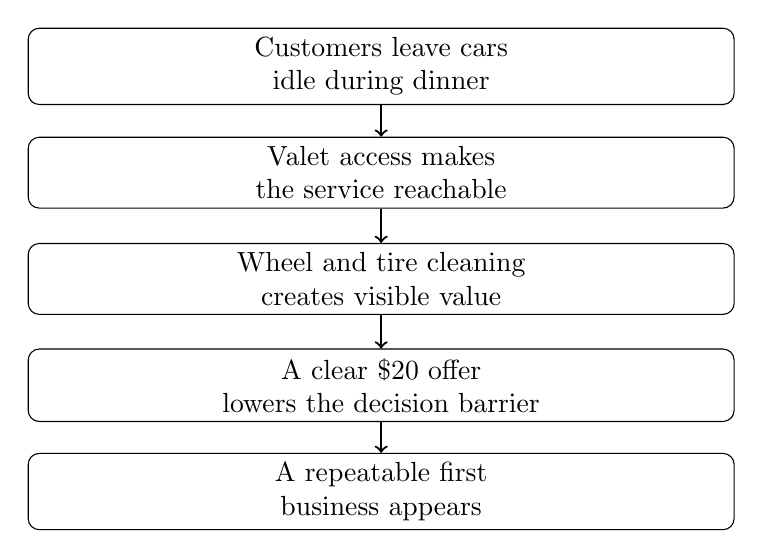
\begin{tikzpicture}[
  box/.style={draw, rounded corners, align=center, text width=0.72\linewidth, minimum height=0.7cm},
  arrow/.style={->, thick}
]
\node[box] (a) at (0,0) {Customers leave cars\\idle during dinner};
\node[box] (b) at (0,-1.35) {Valet access makes\\the service reachable};
\node[box] (c) at (0,-2.7) {Wheel and tire cleaning\\creates visible value};
\node[box] (d) at (0,-4.05) {A clear \(\$20\) offer\\lowers the decision barrier};
\node[box] (e) at (0,-5.4) {A repeatable first\\business appears};
\draw[arrow] (a) -- (b);
\draw[arrow] (b) -- (c);
\draw[arrow] (c) -- (d);
\draw[arrow] (d) -- (e);
\end{tikzpicture}
\caption{Transcript-derived first-business mechanism. No validated screenshot is available for this lecture.}
\end{figure}

\section{Sales As Communication, Not Pressure}

The next question asks about sales. The host frames sales through psychology, and Mark acknowledges the old sales-school world: Zig Ziglar, Tony Robbins, closing, asking for the deal. But he does not make closing the center of his answer. His answer is communication.

The structure is important. Mark says he has energy and confidence, but then he immediately moves to communication. He describes successful salespeople who are not merely salespeople. They are great communicators who love the product or service and believe in it. In his own case, when someone talks with him about Nexalyn technology, brain training, or brain stimulation, they quickly see that he loves what he does. That enthusiasm becomes what he calls a natural sales moment.

We can write the sales mechanism as:
\begin{equation}
\text{sales fit}
\approx
\text{belief}
+
\text{questions}
+
\text{listening}
+
\text{tailored relevance}.
\end{equation}

Again, this is a model of the interview claim, not a literal equation. It helps us see why the pitch does not begin with pressure. It begins with curiosity.

\subsection{Question \& Answer}

\paragraph{Question.}
If sales is psychological, why does Mark avoid making the close the center of the method?

\paragraph{Answer.}
Because, in his account, the psychological work happens before the close. He enters the room asking why the buyer would say no. Then he asks questions, listens to the response, and tailors the message to what the buyer actually needs or cares about. The closing moment is not abolished, but it is demoted. The main operation is matching the message to the person.

A compact update rule captures the motion:
\begin{align}
M_{0} &= \text{initial message},\\
R_{n} &= \text{response to question } n,\\
M_{n+1} &= \operatorname{tailor}(M_{n},R_{n}).
\end{align}

The rule says that the message should not stay fixed after the seller receives information. Listening changes the next version of the pitch. Mark's warning is also negative: do not tell people something they do not want to know, and do not tell them something they already know better than you do.

This is why the medical-professional example matters. In a room of thirty people, he asks how many medical professionals are present. If hands go up, the sales problem changes. He cannot pretend to know health care better than they do. His role becomes humbler: offer a vision of what he thinks could be a better health-care system.

\section{Mentor Advice: Fewer Words, Better Money Habits, More Humility}

The host then asks about the best advice Mark ever received from a mentor. The first answer is verbal discipline: talk too much, slow down, say it in fewer words. The reason is practical. The audience may not know the subject as well as the speaker. Too many words do not necessarily clarify; sometimes they bury the point.

The next answer is finance. Mark warns that entrepreneurs must be careful how they fund businesses and how they spend money, because personal and professional money come together. He gives the concrete image of a good week in the company, a few thousand dollars of business, and then suddenly buying a suit at Saks Fifth Avenue or a \(\$200\) bottle of wine.

The danger can be written as a coupling:
\begin{equation}
\text{early business cash}
\longleftrightarrow
\text{personal spending temptation}.
\end{equation}

In early entrepreneurship, this coupling is strong. The owner feels business momentum personally. A sale becomes a mood. A mood becomes a purchase. The business loses the discipline it needs because the founder spends as if one good week proves the future.

Mark then names humility as a major lesson, not only from a mentor but from life. He frames humility as awareness of what one does not know. In the chapter's logic, humility has already appeared in sales: do not posture before medical professionals. Now it becomes a general operating constraint.

\begin{definition}
In this interview, humility means the active habit of remembering what one does not know, especially while speaking confidently about what one does know.
\end{definition}

That definition keeps together two traits Mark wants to hold simultaneously: confidence and restraint. He does not argue for passivity. He says he is confident and aggressive, but also aware of his limits.

The knowledge-and-wisdom distinction belongs here:
\begin{align}
\text{knowledge} &\approx \text{firsthand experience},\\
\text{wisdom} &\approx \text{listening to people with knowledge}.
\end{align}
Mark says he likes to play in both circles. That phrase bridges the business lesson into the next, more conceptual question.

\section{Trauma, Brain Systems, And The Company Thesis}

The host then introduces a question about trauma through the example of Kanye West, his relationship with his mother, public instability, medication, weight gain, and concern over mental health. The question is not strictly about entrepreneurship, but it connects to Mark's company thesis: how does relationship trauma affect the brain?

Mark begins by defining trauma broadly. Most people, he says, think trauma must be a major event with a major injury. He widens it to anything abnormal in day-to-day life experience. Then he gives a taxonomy:
\begin{equation}
\text{trauma}
\in
\{\text{toxic trauma},\ \text{physical trauma},\ \text{emotional trauma}\}.
\end{equation}

Toxic trauma includes examples such as addiction, alcohol, drugs, food sensitivity, and poisons. Physical trauma includes injuries such as football injuries, bicycle falls, head impacts, traumatic brain injury, and war-related injury. Emotional trauma includes loss of a loved one and betrayal by a loved one.

\begin{figure}
\centering
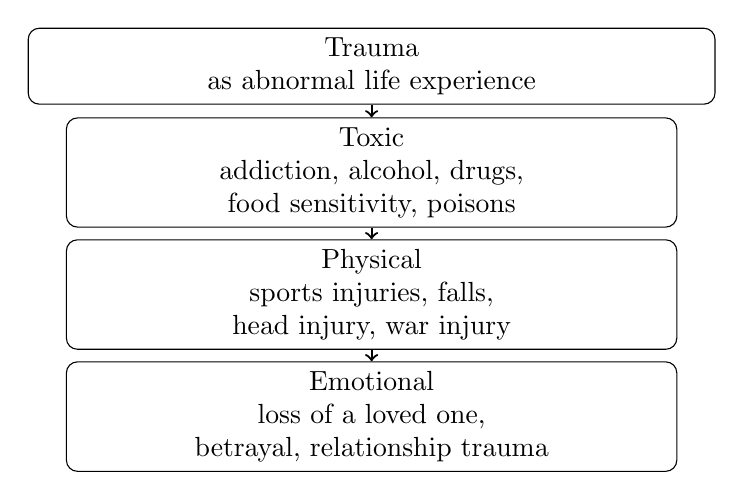
\begin{tikzpicture}[
  box/.style={draw, rounded corners, align=center, text width=0.7\linewidth, minimum height=0.75cm},
  smallbox/.style={draw, rounded corners, align=center, text width=0.62\linewidth, minimum height=0.75cm},
  arrow/.style={->, thick}
]
\node[box] (root) at (0,0) {Trauma\\as abnormal life experience};
\node[smallbox] (toxic) at (0,-1.35) {Toxic\\addiction, alcohol, drugs,\\food sensitivity, poisons};
\node[smallbox] (physical) at (0,-2.9) {Physical\\sports injuries, falls,\\head injury, war injury};
\node[smallbox] (emotional) at (0,-4.45) {Emotional\\loss of a loved one,\\betrayal, relationship trauma};
\draw[arrow] (root) -- (toxic);
\draw[arrow] (toxic) -- (physical);
\draw[arrow] (physical) -- (emotional);
\end{tikzpicture}
\caption{Transcript-derived trauma taxonomy from Mark's explanation.}
\end{figure}

Mark then says some people are relatively unaffected, while for others a little trauma can be devastating. His next claim is a company-worldview claim and should be stated with care: he describes the brain as having two systems, electrical and chemical, which together perform a kind of dance.

\begin{equation}
\text{brain response}
\approx
\text{chemical system}
+
\text{electrical system}.
\end{equation}

The transcript names dopamine, serotonin, and acetylcholine as chemical examples, and EEG frequencies as electrical examples. These details should be preserved because they explain the business thesis, but they should not be expanded into medical doctrine without another source.

\subsection{Question \& Answer}

\paragraph{Question.}
How does Mark connect trauma to a business thesis about brain technology?

\paragraph{Answer.}
He argues that trauma can disturb one or both of the brain systems he cares about: the chemical system and the electrical system. If the disturbance is chemical, medication may be tried. If the disturbance is electrical, he points to EEG frequencies and location in the brain. His company-worldview claim is that treatment should not be only a guessing game of chemically altering a chemically altered brain. He prefers beginning with non-invasive technologies, nutrition, talk therapy or conversation, and foundational life supports.

The progression is:
\begin{enumerate}
\item Trauma creates an overwhelming response.
\item The brain protects the person in the moment through fight or flight.
\item After the trauma, the protective response may not settle back into ordinary balance.
\item The result may appear as stress disorder, chemical imbalance, electrical frequency disturbance, or both.
\item Mark's business claim is that non-invasive approaches and foundational supports should be considered early.
\end{enumerate}

The chapter should preserve the rhythm of this answer. The host asks a concrete question about relational trauma. Mark expands the definition of trauma, classifies it, explains his two-system model, and then turns the model into a critique of trial-and-error medication.

\begin{remark}
The mental-health material in this chapter is interview evidence. It records Mark's explanation of his business worldview. It should not be read as independent medical advice.
\end{remark}

\section{Failure As The Greatest Accomplishment}

After the discussion of trauma and brain health, the host shifts back to career. Mark has started companies and brought a company public. The expected answer to ``greatest accomplishment'' might be wealth, public listing, or scale. Mark gives a different answer: getting up, brushing himself off, licking his wounds, and going back in for another round.

He then makes the point sharper. The worst thing after never having money, he says, is having a lot of money, losing it, and not having any money. He describes watching his life's work loaded into trucks and taken down the road. The decisive figure in the story is his bankruptcy attorney, Nelson Hemsley, who gives him a choice: pay the attorney to clean up the mess, or come to every meeting and every courthouse appearance and face the people to whom he owed money.

The educational mechanism is severe:
\begin{equation}
\text{failure education}
=
\text{loss}
+
\text{accountability}
+
\text{direct exposure to consequences}.
\end{equation}

Mark's greatest accomplishment, in his own telling, was having the strength and nerve to walk into rooms where people hated him because he failed, owed them money, and they lost money. He is careful about the word apology. He does not want to overstate it as a simple apology. He describes being in an apologetic space, giving back what he had, and letting others divide and sell it.

The result, he says, was that on the other side he was a new man. He had a new respect for other people. He remarried his wife and put his family back together. Then the repeated word is humility.

We can summarize the business lesson as a proposition.

\begin{proposition}
In Mark's account, the deepest entrepreneurial education comes when a founder cannot separate business failure from moral consequence.
\end{proposition}

\begin{proof}
The story begins with financial loss, but it does not end there. The attorney's advice forces Mark to remain present before creditors rather than outsourcing the shame. That presence turns failure from a balance-sheet event into a direct encounter with people harmed by the failure. The lesson is therefore not merely that money was lost, but that responsibility had to be faced. Mark names the resulting change humility, and he calls that his greatest accomplishment.
\end{proof}

\section{Structure And Small Wins}

The final movement turns from spectacular failure to ordinary structure. The host asks for self-improvement advice. Mark says, ``Structure.'' He tells a story about a man named Haas who gave him a simple schedule: set the alarm, get out of bed, make the bed, take a shower, be ready for the day, eat lunch and dinner at set times, prepare for bed, and get in bed.

The point of the schedule is not productivity theater. Mark says the reason is that a person needs to be successful at something. The first win may be nothing more than doing what one said one would do. That small kept promise begins to restore self-trust.

We can write the update rule as:
\begin{align}
S_{0} &= \text{one small promised action},\\
C_{n} &= \begin{cases}
1, & \text{if the promise is kept on day } n,\\
0, & \text{if it is not kept on day } n,
\end{cases}\\
H_{n+1} &= H_{n} + \alpha C_{n},
\end{align}
where \(H_{n}\) denotes confidence in one's own follow-through and \(\alpha>0\) is the gain from keeping a promise. This is a schematic rule, not psychology by equation. Its purpose is to preserve the practical logic: success at one small thing can become the next unit of structure.

\begin{figure}
\centering
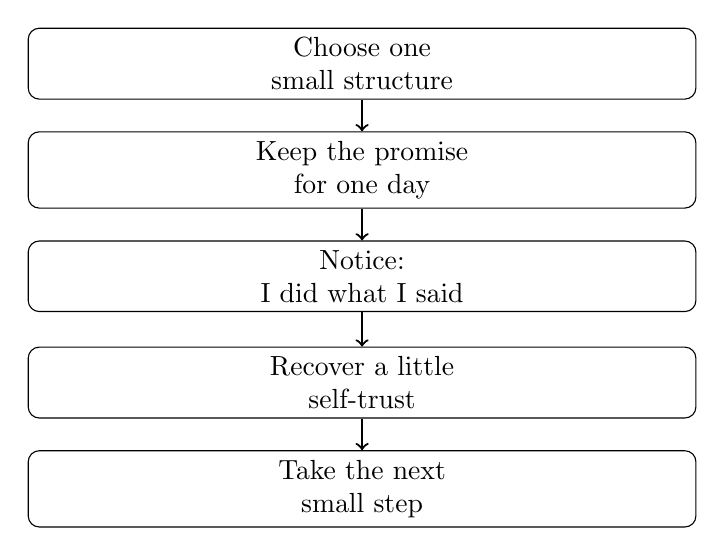
\begin{tikzpicture}[
  box/.style={draw, rounded corners, align=center, text width=0.68\linewidth, minimum height=0.75cm},
  arrow/.style={->, thick}
]
\node[box] (a) at (0,0) {Choose one\\small structure};
\node[box] (b) at (0,-1.35) {Keep the promise\\for one day};
\node[box] (c) at (0,-2.7) {Notice:\\I did what I said};
\node[box] (d) at (0,-4.05) {Recover a little\\self-trust};
\node[box] (e) at (0,-5.4) {Take the next\\small step};
\draw[arrow] (a) -- (b);
\draw[arrow] (b) -- (c);
\draw[arrow] (c) -- (d);
\draw[arrow] (d) -- (e);
\end{tikzpicture}
\caption{Transcript-derived small-wins ladder.}
\end{figure}

Mark warns against the New Year's resolution pattern: deciding to stop A, B, C, and D, start E, F, G, and H, then failing early and retreating into old habits. The alternative is smaller and more durable. Drink water. Take a walk. Be on time to work. Set the alarm. Get out of bed. Say hello and smile. The point is not that these actions solve everything. The point is that they create a first successful unit of self-command.

\section{Summary}

The interview moves in a clean entrepreneurial arc. It begins with a public-company CEO and then goes backward to a first small business: idle cars, visible improvement, and a clear \(\$20\) offer. It moves from starting to selling, where Mark replaces pressure with communication, questions, listening, and humility before expertise. It then turns to mentor advice: fewer words, more careful money habits, and humility as a working discipline.

The middle of the interview broadens into Mark's company worldview about trauma, chemical and electrical brain systems, EEG frequencies, and the limits of trial-and-error medication. Those claims should remain explicitly sourced to the interview. The final third returns to entrepreneurship through failure: the greatest accomplishment is not merely going public, but facing creditors, learning from consequence, and emerging with humility. The closing advice brings the same principle down to daily scale. We do not rebuild a life by declaring total transformation. We begin with one kept promise, notice it, and let the next step become possible.